% Mini Project. Thesis presentation
% By : 	Neelamadhav Gantayat,
%.


\documentclass[xcolor=dvipsnames]{beamer}
\setbeamertemplate{bibliography item}[text]
\usepackage{amsfonts}
\usepackage{amsthm}
\usepackage{amsmath}
\usepackage{verbatim}

\usepackage{epsfig}

\usepackage{tikz}
\usepackage{etex}
\usepackage{mdwlist}

\hypersetup{colorlinks,%
            citecolor=black,%
            filecolor=black,%
            linkcolor=black,%
            urlcolor=black,%
            pdftex}

%\usepackage{gastex}
\usepackage[latin1]{inputenc}
\usepackage[T1]{fontenc}
\usepackage{lmodern}
%\usepackage{algorithm}
%\usepackage{algorithmic}
% \usepackage{multirow}
\usepackage{multicol}
\usepackage{listings}
\usepackage{color, colortbl}


\definecolor{Green}{rgb}{0.3,3,0.3}
%\usepackage{flexiprogram}

%\setbeamertemplate{navigation symbols}{}
\setbeamercolor{frametitle}{fg=red!85!black,bg=white}
\setbeamercolor{title}{fg=red!85!black,bg=white}
\usetheme{CambridgeUS}
\lstset{frame=shadowbox, rulesepcolor=\color{black}, captionpos=b}

%\beamersetuncovermixins{\opaqueness<1>{25}}{\opaqueness<2->{15}}

% \AtBeginSubsection[]
%{
%  \begin{frame}<beamer>
%    \frametitle{Outline}
    %\tableofcontents[currentsection,currentsubsection]
%  \end{frame}
%}

%\AtBeginSection[]
%{
%  \begin{frame}<beamer>
%    \frametitle{Outline}
%    {\tableofcontents[currentsection]}
%%       \setcounter{tocdepth}{1}
%  \end{frame}
%}

\begin{document}
%\usebackgroundtemplate{
%\includegraphics[width=\paperwidth,
%height=\paperheight]{background}
%} 


	\title[Sanskrit Sandhi]{\textsc{Sanskrit sandhi splitting and merging tools}}
	\author[Shubham, Neelamadhav]{Shubham Bhardwaj \\ Neelamadhav Gantayat\\ \small{(Mini Project)} \\   \small{under the guidance of} \\ 
	\large{Prof. Rahul Garg \\ Prof. Sumeet Agarwal}}
	
% 	\titlegraphic{\includegraphics[scale=0.5]{logo.png}}
	
	\institute[IIT Delhi]{ \\}
	\date[\today]{\today}
	
 \begin{frame}
   
 	\titlepage
 
 \end{frame}
 
 
 \begin{frame}
 \frametitle{Outline}
      {\tableofcontents}
 \end{frame}
 

\section{Sandhi}
\begin{frame}
\frametitle{Sandhi}
\begin{figure}
	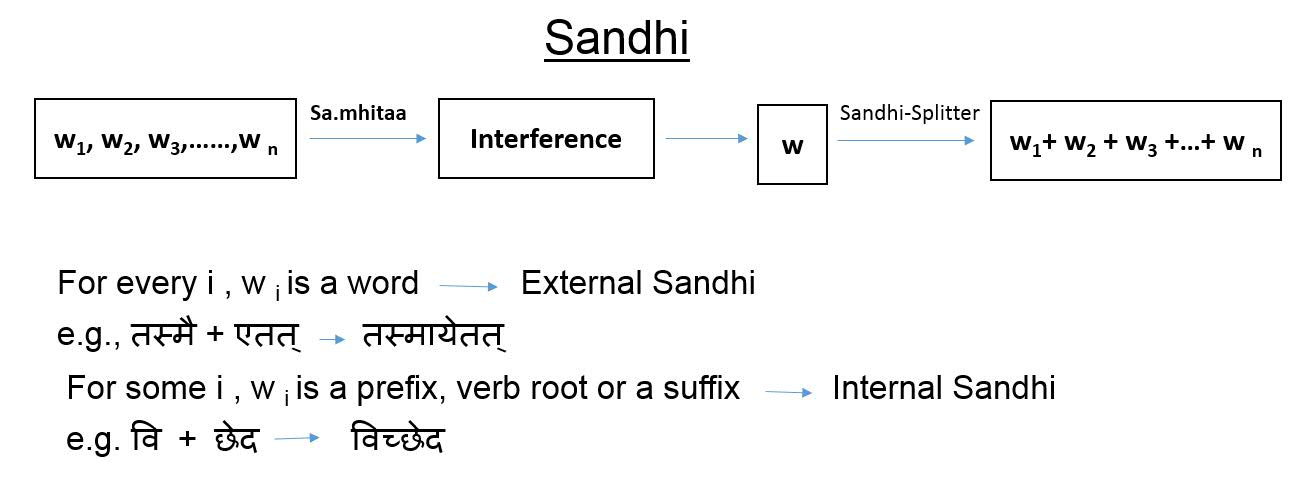
\includegraphics[scale=0.35]{img/sandhi.png} 
 \end{figure}
\end{frame}

\subsection{What governs this interference?}
\begin{frame}
\frametitle{What governs this interference?}
\begin{figure}
	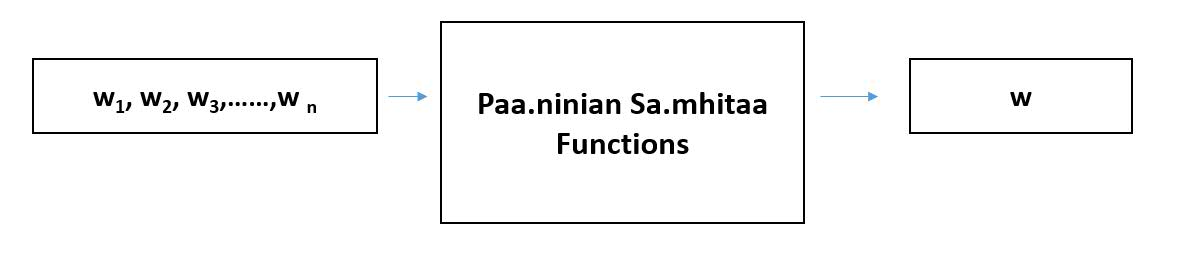
\includegraphics[scale=0.35]{img/panini.png} 
 \end{figure}
\begin{itemize}
\item A.s.taadhyaayii of Paa.nini
\item Sa.mhita governs sutras 73-157 of Chapter 1 of Book 6 and all sutras of Chapter 3 and 4 of Book 8
\item Total number of Paa.ninian Sandhi Sutras - 271
\item Paa.ninian Sutras codified in the form of Sets and Functions

\end{itemize}
\end{frame}

\begin{frame}
\frametitle{Automatic Evaluation of Sandhi Splitters and Generators}
\begin{itemize}
\item Sanskrit Sandhi Analyzer and Generator\footnote{\url{http://sanskrit.jnu.ac.in/sandhi/viccheda.jsp?itext=}}
    \\(Dr. G.N. Jha, Special Centre for Sanskrit Studies, JNU)

\item Sandhi-Splitter and Generator\footnote{\url{http://52.25.246.194/scl/}} 
   \\(Dr. Amba Kulkarni, Department of Sanskrit Studies, University of Hyderabad)

 \item The Sanskrit Reader Companion and the Sandhi Engine\footnote{\url{http://sanskrit.inria.fr/DICO/reader.fr.html}}
    \\(Dr. Gerard Huet ,Computational Linguistics, INRIA, France)

%\item Any more that you are aware of
\end{itemize}
\end{frame}

\subsection{Sandhi Corpus}
\begin{frame}
\frametitle{Sandhi Corpus}
\begin{itemize}
\item 40 different sandhi-split corpora available on the University of Hyderabad website\footnote{\url{http://sanskrit.uohyd.ac.in/Corpus/}} 
\item Problems - Insufficient splits, no splits, wrong splits, typos
\begin{center}
\begin{tabular}{ l l }
\textbf{Text (first 100 cases)} & \textbf{Errors}\\
 Vinodini &  42\% \\ 
 Manjusa &   44\% \\  
 Vyutpattivada & 58\%   \\
 Dutvakyam & 8\% \\
 Short-stories & 9\% \\
\end{tabular}
\end{center}
\item Creating a Srimad Bhagvad Gita Corpus
\end{itemize}
\end{frame}



\section{Sanskrit Transliteration}

\subsection{Need for a transliteration tool}
\begin{frame}
\frametitle{Need for a transliteration tool}
\begin{itemize}
\item Various data sources of Sanskrit literature were encoded in different scripts.
\item Different tools use different transliteration schemes for input and output

\item From our survey identified some web tools and some standalone tools - No bulk conversion option
\item Need a tool which can convert from one script to another in bulk (Files and folders)
%\item Wrote a new sanskrit transliteration tool.
\end{itemize}
\end{frame}

\subsection{Sanskrit Transliteration}


\begin{frame}
\frametitle{Sanskrit Transliteration}
\begin{figure}
	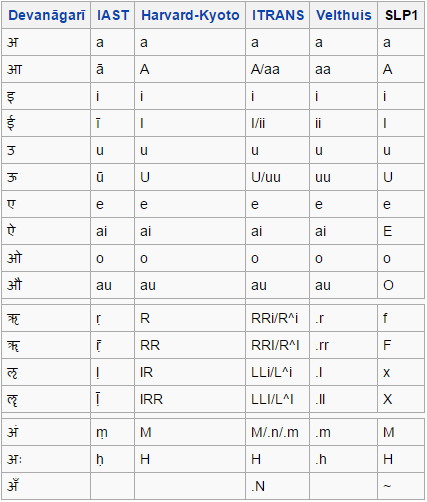
\includegraphics[scale=0.35]{img/transliteration.png} 
 	\caption{\tiny{Example: One step conversation\footnote{\url{https://en.wikipedia.org/wiki/Devanagari_transliteration}}}}
 \end{figure}
 
 \begin{itemize}
 %\item Some of the scripts for Sanskrit.
 \item Among these SLP1 script has complete encoding scheme for Devanagari
  
  
 \end{itemize}
 
\end{frame}



\section{Sandhi Corpus Format}
\begin{frame}
\frametitle{Sandhi Corpus Format}
\begin{itemize}
\item Manually curated corpus from University of Hyderabad \footnote{\url{http://sanskrit.uohyd.ac.in/Corpus/}} 
\end{itemize}
Formats\
\begin{itemize}
\item Single words split into multiple words
\begin{figure}
	
\includegraphics[scale=0.5]{img/singleword.png} 
 \end{figure}
\item Multiple words split into multiple words
\begin{figure}
	
\includegraphics[scale=0.5]{img/multiword.png} 
 \end{figure}
\item Multiple words span across multiple lines
\begin{figure}
	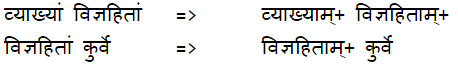
\includegraphics[scale=0.5]{img/multiline.png} 
 \end{figure}
\end{itemize}
\end{frame}

%\subsection{Problems with the corpus}
%\begin{frame}
%\frametitle{Problems with the corpus}
%\begin{itemize}
%\item Wrong split
%\item No split
%\item typo mistakes
%\end{itemize}
%solution
%\begin{itemize}
%\item Manually look into the splits
%\item Check for the split words in the dictionary
%\end{itemize}
%\end{frame}

\subsection{Processing corpus}
\begin{frame}
\frametitle{Processing corpus}
\begin{itemize}
\item Filtered out single word, multi split instances
\item Combined multi lines into single line and converted them to multi word instance.
\item One way of ensuring correctness is checking for the split words in the dictionary
\end{itemize}
\end{frame}

\section{Dictionary Creation}
\begin{frame}
\frametitle{Dictionary Creation}
Various types of dictionary, example: \footnote{\url{http://www.sanskrit-lexicon.uni-koeln.de/}}
\begin{itemize}
\item Sanskrit to Sanskrit dictionary
\item Sanskrit to English dictionary
\item English to Sanskrit dictionary
\end{itemize}
Dictionary words creation
\begin{itemize}
\item Parsed ``Sanskrit to Sanskrit'' and ``Sanskrit to English'' 
\item Created a comprehensive list of words from all the dictionary.
\end{itemize}
\end{frame}

\begin{frame}
\frametitle{Filtering Corpus}
\begin{itemize}
\item Identified all the sandhi splits from the corpus where all the split words are available in the dictionary
\item out of 97674 samples we identified 15325 samples where all the splits are present in the dictionary
\end{itemize}
\end{frame}

\section{Online Sandhi Tools}

%\begin{frame}
%\frametitle{Online Sandhi Tools}
%\begin{itemize}
%\item jnu \url{http://sanskrit.jnu.ac.in/sandhi/viccheda.jsp?itext=}
%\item inria \url{http://sanskrit.inria.fr/DICO/reader.fr.html}
%\item uoh \url{http://52.25.246.194/scl/}
%\end{itemize}
%\end{frame}

\subsection{Evaluation}
\begin{frame}
\frametitle{Evaluation}
\begin{itemize}
%\item jnu 28/158
%\item uoh 125/158
%\item inria - 

\item Sanskrit Sandhi Analyzer and Generator - 1523/7217 (21.10\%)

\item Sandhi-Splitter and Generator - 4248/7217 (58.86\%)

 \item The Sanskrit Reader Companion and the Sandhi Engine - Not yet done

\end{itemize}
\end{frame}

\begin{frame}
\frametitle{Future Work}
\begin{itemize}
\item Validate dictionary output
\item Check for Sandhi splitting and Sandhi Merging tools apart from the above three
\item Create corpus using Sandhi Merging tool by merging words or dictionary.
\item Manually create Sandhi corpus from ``Sri Mad Bhagwat Gita''
\item Create our own Merging and splitting tool if required.
\end{itemize}
\end{frame}
\end{document}
